% !TEX root = ../../my-thesis.tex
% TODO: replace `\textbf` by `\textbf`
% replace assets/ by ""
\graphicspath{{./content/chap1_diff_in_graphs/figures/}}

\setcounter{equation}{0}
\setcounter{figure}{0}
\setcounter{table}{0}
% \setcounter{page}{1}
\makeatletter % changes the catcode of @ to 11
\renewcommand{\thetable}{S\arabic{table}}
\renewcommand{\theequation}{S\arabic{equation}}
\renewcommand{\thefigure}{S\arabic{figure}}
\makeatother % changes the catcode of @ back to 12

\section{Supplementary Note}
    \label{secSI:supmat}
    % We justify heuristically why population dynamics can be investigated analytically with a deterministic approximation, but on the other hand Monte Carlo simulations of the stochastic process are necessary to investigate neutral diversity metrics.

    \subsection{Mathematical construction of the model}\label{secSI:formal_descrip}
    The model is a measure-valued point process \cite{Bansaye2015}, so that individuals are represented as dirac functions $\delta_{x_{k}^{(i)}}$, where $x_{k}^{(i)} \in \mathcal{X}$ corresponds to the traits' value of individual $k$ located on vertex $v_i$.
    %
    Under this formalism, the population on $v_i$ is represented as a sum of dirac functions $\nu^{(i)} = \sum^{N^{(i)}}_k \delta_{x_{k}^{(i)}}$, where $N^{(i)}$ is the local population size. 
    %
    It follows that the time variation of the process can be described by the so-called infinitesimal generator $L$, defined for all real valued functions $\phi$ as
    \begin{equation}\label{eqSI:def_infgen}
         L \phi(\nu^{(i)}_t) = \partial_t \E \left[\phi(\nu^{(i)}_t) \right]
    \end{equation}
    (see \cite{Linke2015} for an introduction to infinitesimal generators). \Cref{eqSI:def_infgen} provides the expected time variation at time $t$ of e.g. the population size by choosing $\phi(\nu^{(i)}_t) = \int_\mathcal{X} \nu^{(i)}_t(dx)$.
    %
    Recall that we use
    $b^{(i)}$ to denote the birth rate on vertex $v_i$,
    $d$ for the death rate,
    $\mu$ for the mutation probability,
    $m$ for the migration probability,
    $\mathcal{M}(x,y) = \frac{1}{\sqrt{2\pi}\sigma_\mu} \exp \left(\frac{||x-y||^2}{2\sigma_\mu} \right)$ for the mutation kernel,
    $K$ for the local carrying capacity,
    $A = (a_{i,j})_{1\leq i, j \leq M}$ for the adjacency matrix of the graph $G$, and
    $D = (d_1,d_2,\dots,d_M)$ for the vector containing the degree of each vertex.
    %
    In order to explicitly write the generator $L$,
    let us recall that five events of different natures can alter the number of individuals with trait $x$ on vertex $v_i$:
    \begin{itemize}
        \item an individual on $v_i$ with trait $x$ can give birth to an offspring that does not experience mutations nor migration, at rate $(1 - \mu ) (1 - m) b^{(i)}(x)$,
        \item an individual on $v_i$ with trait $y$ can give birth to an offspring with mutated trait $x$ that does not experience migration, at rate $\mu (1-m) \mathcal{M}(x,y) b^{(i)}(y)$,
        \item an individual on $v_i$ with trait $x$ can die, at rate $d(N^{(i)}) = \frac{N^{(i)}}{K} = \frac{1}{K} \int_\mathcal{X} \nu_t^{(i)} (dx)$,
        \item an individual on $v_j$ with trait $x$ can give birth to an offspring that does not experience mutations and migrates to $v_i$, at rate $ \frac{a_{i,j}}{d_j} (1 - \mu ) m \, b^{(j)}(x)$,
        \item an individual on $v_j$ with trait $y$ can give birth to an offspring with mutated trait $x$ that migrates to $v_i$, at rate $ \frac{a_{i,j}}{d_j} \mu  m \mathcal{M}(x,y) b^{(j)}(x)$.
    \end{itemize}
     %
    Summing over all all individuals and all vertices yields
    \small
    \begin{align} \label{eqSI:infinitesimal_generator}
        L\phi(\nu^{(i)}_t) &= \int_\mathcal{X} \left\{ b^{(i)}({\textbf x}) (1 - \mu ) (1 - m)( \phi(\nu^{(i)}_t + \delta_{{\textbf x}}) - \phi(\nu^{(i)}_t))\right\} \nu^{(i)}_t(d{\textbf x}) &\text{ births w/o mutations, w/o migrations} \nonumber\\
        &\quad + \int_\mathcal{X}  \left\{\mu (1-m) \int_\mathcal{X} b^{(i)}(y) (\phi(\nu^{(i)}_t + \delta_z) - \phi(\nu^{(i)}_t))\mathcal{M}({\textbf x},y) dy \right\} \nu^{(i)}_t(d{\textbf x})  &\text{ births w/ mutations, w/o migrations} \nonumber\\
        &\quad + \iint_\mathcal{X} \left\{ \frac{1}{K}(\phi(\nu^{(i)}_t - \delta_{{\textbf x}})) - \phi(\nu^{(i)}_t))\nu^{(i)}_t(d y) \, \nu^{(i)}_t(dx)  \right\} &\text{ deaths} \nonumber\\
        &\quad + \sum_{j \neq i } \frac{a_{i,j}}{d_j} \int_\mathcal{X}  \mu m \left\{ \int_\mathcal{X} b^{(j)}(y) (\phi(\nu^{(j)} +  \delta_{\textbf x}) - \phi(\nu^{(j)}))\mathcal{M}({\textbf x}, y)dy \right\} \nu^{(j)}_t(d{\textbf x})  &\text{ migrations w/ mutations} \nonumber\\
        &\quad + \sum_{j\neq i}\frac{a_{i,j}}{d_j} \int_\mathcal{X} \left\{ b^{(j)}({\textbf x}) (1 - \mu ) m ( \phi(\nu^{(j)} + \delta_{{\textbf x}}) - \phi(\nu^{(j)})) \right\} \nu^{(j)}_t(d{\textbf x}). &\text{ migrations w/o mutations} 
    \end{align}
    \normalsize
    %
    Taking expectations in \cref{eqSI:infinitesimal_generator}, one can obtain an equation for the mean trajectory of the quantity of interest, $ \E \left[ \phi(\nu^{(i)}_t) \right]$. Nonetheless, \cref{eqSI:infinitesimal_generator} involves an integral with respect to $\nu^{(i)}_t(dx) \nu^{(i)}_t(dy)$, making it impossible to obtain an explicit solution. It is therefore unclear whether one can gain insight into the stochastic dynamics from \cref{eqSI:infinitesimal_generator} without simplifying assumptions. We refer to \cite{Champagnat2006} for a detailed discussion on the topic.
    
    \subsection{Deterministic approximation} 
    One strategy to overcome the difficulties encountered above is to assimilate the process to its mean trajectory, assuming that $\E \left[ \nu^{(i)}_t \right] \approx \nu^{(i)}_t$ and further approximating $\nu^{(i)}_t$ with a continuous deterministic function $n_t^{(i)}$. Such strategy inherently neglects the stochasticity of the process, which is reasonable provided that a force dampens the stochastic fluctuations of the quantity of interest.
    
    \subsubsection{Setting with no selection}
    Consider a setting with no selection and recall that in this setting where $x \equiv u \in \mathcal{X} = \mathcal{U}$ we define
    \begin{equation}\label{eqSI:b_d_sett1}
      b^{(i)}(x) \equiv b 
    \end{equation}
    By applying the strategy mentioned above and choosing $\phi(n^{(i)}_t) = \int_\mathcal{X} n^{(i)}_t(x) dx$, \cref{eqSI:infinitesimal_generator} transforms into the deterministic approximation of the population size dynamics given in the main-text by
    \begin{equation}\label{eqSI:sett1_popdyn_simple}
      \partial_t N_t^{(i)} = N_t^{(i)} \left[ b(1-m) - \frac{N_t^{(i)}}{K} \right] +  m b \sum_{j\neq i}\frac{a_{i,j}}{d_j}  N_t^{(j)} .
    \end{equation}
    Competition stabilises the population size dynamics, which behaves deterministically. This is supported by \cref{figSI:pde-vs-IBM-trans-setting1_localpop}a, which shows how \cref{eqSI:sett1_popdyn_simple} accurately describes the population size for varying migration regimes. Nonetheless, stochastic fluctuations drive the dynamics of the neutral trait distribution. Attempting to characterise the neutral trait distribution with the same strategy, this time setting $\phi(n^{(i)}_t) = n^{(i)}_t(u)$, yields
    %
    \begin{equation}\label{eqSI:detern_approx_infgen_sett1}
    \begin{split}
    \partial_t n_t^{(i)}(u) &= n_t^{(i)}(u)\left[b(1-m)(1-\mu) - \frac{1}{K}\int_\mathcal{U} n_t^{(i)}({\textbf u}) \, d {\textbf u})\right] \\
    &\quad + (1- m)\mu b \int_\mathcal{U} \, n_t^{(i)}( {\textbf u})  \mathcal{M}( u, {\textbf u}) \, d{\textbf u} \\
    &\quad + m \mu b \sum_{j\neq i}\frac{a_{i,j}}{d_j}  \int_\mathcal{U} \,  n_t^{(j)}(u) \mathcal{M}( u, {\textbf u}) d{\textbf u}\\
    &\quad + m (1 - \mu) b \sum_{j\neq i}\frac{a_{i,j}}{d_j} b \, n_t^{(j)}(u).
  \end{split}
\end{equation}
%
Solving for \cref{eqSI:detern_approx_infgen_sett1}, one can show that the variance of $n_t^{(i)}$ continuously grows in time (see \cref{figSI:pde-vs-IBM-trans-setting1_localpop}) and tends to infinity as time goes to infinity, which is an unrealistic behaviour considering finite populations. Intuitively, this reflects the fact that no stabilising force acts on the neutral trait distribution, such that random fluctuations play a major role in driving the dynamics of the stochastic process.
%
\Cref{figSI:pde-vs-IBM-trans-setting1_localpop} shows how IBM trajectories significantly differ from \cref{eqSI:detern_approx_infgen_sett1}, and \cref{figSI:pde-vs-IBM-mresponse-setting1} illustrates how diversity metrics obtained from \cref{eqSI:detern_approx_infgen_sett1} do not match those obtained from simulations of the IBM.

\subsubsection{Setting with heterogeneous selection}\label{sec:anal_sett_2}
In contrast to the neutral trait dynamics, the adaptive distribution can successfully be approximated by a deterministic description because selection pressure acts as a stabilising force and stabilises the populations' adaptive trait, dampening the stochastic fluctuations.
%
Consider the setting with heterogeneous selection and recall that in this setting where $x \equiv (s,u) \in \mathcal{X} = \mathcal{S} \times \mathcal{U}$ we define
\begin{equation}\label{eqSI:b_d_sett2}
  b^{(i)}(x) \equiv b(1-p(s-\theta_i)^2).
\end{equation}
%
By applying the same strategy as above to characterise the adaptive trait distribution $n^{(i)}_t(s)$ by choosing $\phi(n^{(i)}_t) = n^{(i)}_t(s) \equiv \int_\mathcal{U} n^{(i)}_t(u,s) du $, \cref{eqSI:infinitesimal_generator} transforms into
%
\begin{equation}\label{eqSI:general_equation}
    \begin{split}
    \partial_t n_t^{(i)}(s) &= n_t^{(i)}(s)\left[b^{(i)}(s)(1-m)(1-\mu) - \frac{1}{K}\int_\mathcal{S} n_t^{(i)}({\textbf s}) \, d {\textbf s})\right] \\
    &\quad + (1- m)\mu \int_\mathcal{S} b^{(i)}({\textbf s}) \, n_t^{(i)}( {\textbf s})  \mathcal{M}({\textbf s}, s) \, d{\textbf s} \\
    &\quad + m \mu \sum_{j\neq i}\frac{a_{i,j}}{d_j}  \int_\R b^{(j)}({\textbf s}) \,  n_t^{(j)}(s) \mathcal{M}({\textbf s}, s) d{\textbf s}\\
    &\quad + m (1 - \mu) \sum_{j\neq i}\frac{a_{i,j}}{d_j}  b^{(j)}(s) \, n_t^{(j)}(s).
  \end{split}
\end{equation}
%
Assuming that the variance of the mutation kernel is small, one can use a diffusion approximation for the mutation term \cite{Kimura1965,Debarre2013,Mirrahimi2020}
\begin{equation}
  \begin{split}
  \int_\mathcal{S} b^{(i)}({\textbf s}) \, n_t^{(i)}({\textbf s}) \mathcal{M}({\textbf s}, s) \, d{\textbf s} 
          &= b^{(i)}(s,t) \, n_t^{(i)}(s) + \tfrac{1}{2} \sigma_\mu^2 \Delta_s ( b^{(i)} n_t^{(i)})(s) .
  \end{split}
\end{equation}
%
Neglecting the terms in $m \mu$, we obtain
%
\begin{equation}
  \begin{split}
    \partial_t n_t^{(i)}(s) &= n_t^{(i)}(s)\left[b^{(i)}(s,t)(1-m - \mu) - \frac{1}{K} \int_\mathcal{S} n_t^{(i)}({\textbf s}) \, d {\textbf s})\right] \\
    & \quad + \mu \left[ b^{(i)}(s,t) \, n_t^{(i)}(s) + \tfrac{1}{2} \sigma_\mu^2 \Delta_s (b^{(i)} n_t^{(i)})(s) \right] \\
    & \quad + m \sum_{j \neq i} b^{(j)}(s,t) n_t^{(j)}(s) a_{i,j}
    \end{split}
\end{equation}
which, after rearranging terms, yields the elegant deterministic approximation of the adaptive trait dynamics
%
\begin{equation}\label{eqSI:PDE_adapt}
  \partial_t n_t^{(i)}(s) =n_t^{(i)} (s) \left[b^{(i)}(s)(1-m) -  \frac{1}{K}\int_\mathcal{S}  n_t^{(i)}({\textbf s}) d{\textbf s}  \right] + m \sum_{j\neq i} b^{(j)}(s) \frac{a_{i,j}}{d_j} n_t^{(j)}(s) + \tfrac{1}{2} \mu \sigma_\mu^2 \Delta_s \left[ b^{(i)}(s) n^{(i)}_t(s) \right].
\end{equation}
%
Setting $m = 0$ \cite{Mirrahimi2020} shows that \cref{eqSI:PDE_adapt} admits a stationary solution that is Gaussian, with variance $ \nicefrac{\sqrt{\mu} \sigma_\mu^2}{\sqrt{p}}$. 
%
Therefore, the variance of the adaptive trait distribution stabilises to a finite value. Intuitively, this reflects the fact that the random fluctuations of the adaptive trait distribution are dampened by the stabilising force of selection. Provided that the selection strength $p$ is large enough, \cref{eqSI:PDE_adapt} is a good approximation of the adaptive trait distribution obtained from the stochastic process.
%
\Cref{figSI:pde-vs-IBM-trans-setting2_localpop} shows how IBM trajectories are similar to the ones obtained from \cref{eqSI:detern_approx_infgen_sett1}, and \cref{figSI:pde-vs-IBM-mresponse-setting2} illustrates how diversity metrics obtained from \cref{eqSI:detern_approx_infgen_sett1} match those obtained from simulations of the IBM.


\subsection{Trait-dependent competition}\label{secSI:trait-dep-comp}
To test whether the effects of the metrics hold under more complex ecological processes, we designed an extra experiment considering heterogeneous selection and adaptive trait-dependent competition, where the death rate of individuals on $v_i$ with traits $x_k^{(i)} = (u_k^{(i)}, s_k^{(i)}) \in \mathcal{U} \times \mathcal{S}$ is given by
\begin{equation}
    d(x_k^{(i)}, \nu^{(i)}) = \frac{1}{K}\int_{\mathcal{S}} \exp\Bigl(-\frac{(s_k^{(i)} - {\textbf s})^2}{2\sigma_\alpha^{2}} \Bigr) \nu^{(i)}({\textbf s})
\end{equation}
where $\sigma_\alpha$ is the competition bandwidth.
This competition kernel tends to increase the population size, as it decreases the overall competition. The adaptive dynamics theory predicts that when $m = 0$, competition promotes two distinct types of individuals at either side of the adaptive trait optimum for a competition bandwidth $\sigma_\alpha < \nicefrac{1}{\sqrt{2p}}$, while a single type is observed when $\sigma_\alpha > \nicefrac{1}{\sqrt{2p}}$ \cite{DoebeliMichael2011Ad}.
We performed simulations in both cases for graphs with $M=7$ vertices and show results of the multivariate regression analyses in \cref{tableSI:coefficients_trait-dep-comp}.
The analyses demonstrate that the trends reported in the main manuscript remain unchanged in both cases.

% \subsection{Variance partitioning}\label{secSI:variance_partitioning}
% We demonstrate that the neutral differentiation measure $Q_{ST,u}$ and the adaptive differentiation measure $Q_{ST,s}$ used in the study correspond to the original measure of genetic differentiation for quantitative traits in \cite{Lande1992,WHITLOCK2008}, denoted by $Q_{ST}$ for $Q$-statistics, for a haploid population.
% The definition of the neutral differentiation $Q_{ST,u}$ used in the study is given in \cref{eq:def_Qsty} by
% \begin{equation}\label{eqSI:QST_def}
%     Q_{ST,u} = \nicefrac{\sigma^2_{B,u}}{\sigma^2_{M,u}},
% \end{equation}
% where $\sigma^2_{B,u} = \E \left[\frac{1}{M} \sum_{i} \left(\bar{u}^{(i)} - \bar{u}\right)^2 \right]$ denotes the expected neutral trait variance between the vertices and $\sigma^2_{M,u} = \E \left[ \frac{1}{M} \sum_i \frac{1}{N^{(i)}} \sum_k \left( u_{k}^{(i)} - \bar{u}\right)^2 \right]$ denotes the expected neutral trait variance in the metapopulation.
% % 
% % and $\bar{x}^{(i)} = \tfrac{1}{N^{(i)}} \int_\mathcal{X} x \, \nu^{(i)}(dx)$  is the trait mean on $v_i$. 
% %%
% For a haploid population, \cite{WHITLOCK2008} defines $Q_{ST}$ as
% \begin{equation}\label{eqSI:QST_original_def}
%     Q_{ST,u} = \nicefrac{\sigma^2_{B,u}}{(\sigma^2_{W,u}+\sigma^2_{B,u})},
% \end{equation}
% where $\sigma^2_{W,u} =  \frac{1}{M} \sum_{i}^M \E \left[ \frac{1}{N^{(i)}} \sum_k  \left(u_k^{(i)} - \bar{u}^{(i)}\right)^2 \right]$ denotes the average expected neutral genetic variance within vertices. We now show that $\sigma^2_{W,u} + \sigma^2_{B,u} = \sigma^2_{M,u}$, so that \cref{eqSI:QST_def} is equivalent to \cref{eqSI:QST_original_def}.
% %
% % and the neutral trait variance as $\Var_u(\nu^{(i)}) = \tfrac{1}{N^{(i)}} \int_\mathcal{X} u^2 \nu^{(i)} (dx) - \left[\bar{u}^{(i)}\right]^2$.
% By adopting the notations introduced in \cref{secSI:formal_descrip} we have 
% \begin{equation}
%     \begin{split}
%       \sigma^2_{W,u} &=  \E \left[ \frac{1}{M} \sum_{i}^M  \frac{1}{N^{(i)}} \sum_k  \left(u_k^{(i)} - \bar{u}^{(i)}\right)^2 \right] \\
%               &= \frac{1}{M}\sum_{i}^M \E \left[ \frac{1}{N^{(i)}}\int_\mathcal{X} \left[x - \bar{x}^{(i)}\right]^2 \nu^{(i)}(dx) \right]\\
%                 &=\frac{1}{M}\sum_{i}^M \E \left[ \frac{1}{N^{(i)}} \int_\mathcal{X}  x^2  \nu^{(i)}(dx)  - 2  \bar{x}^{(i)} \int_\mathcal{X}  x \nu^{(i)}(dx) + \left( \bar{x}^{(i)}\right) ^2 \right]\\
%                 &= \frac{1}{M}\sum_{i}^M \E \left[ \frac{1}{N^{(i)}} \int_\mathcal{X} x^2 \nu^{(i)}(dx) - \left( \bar{x}^{(i)} \right) ^2 \right],
%       \end{split}\label{eqSI:def_alpha}
% \end{equation}
% \begin{equation}
%     \begin{split}
%       \sigma^2_{W,u} &= \E \left[ \frac{1}{M} \sum_i \frac{1}{N^{(i)}} \sum_k \left( u_{k}^{(i)} - \bar{u}\right)^2 \right]\\
%       &= \frac{1}{M} \sum_{i} \E \left[ \left(\bar{u}^{(i)} - \bar{u}\right)^2 \right] \\
%         &= \frac{1}{M} \sum_{i=1}^{M} \E \left[ \left[ \bar{x}^{(i)} - \bar{x} \right]^2 \right]\\
%         &= \frac{1}{M} \sum_{i=1}^{M} \E \left[ \left[\bar{x}^{(i)}\right]^2 - \bar{x}^2 \right],
%     \end{split}\label{eqSI:def_beta}
% \end{equation}
% and
% \begin{equation}
%   \begin{split}
%     \sigma_{T,u}^2 &= \E \left[ \frac{1}{M} \sum_i^{M} \frac{1}{N^{(i)}} \int_\mathcal{X} \left(x - \bar{x} \right)^2 \nu^{(i)}(dx) \right] \\
%              &= \frac{1}{M} \sum_i^{M} \E \left[ \left[\frac{1}{N^{(i)}} \int_\mathcal{X} x^2 \nu^{(i)}(dx)\right] - \bar{x} ^2 \right]
%   \end{split}\label{eqSI:def_gamma}
% \end{equation}

% Adding \cref{eqSI:def_alpha} to \cref{eqSI:def_beta}, we obtain \cref{eqSI:def_gamma} and therefore recover \cref{eqSI:QST_original_def} from \cref{eqSI:QST_def}.

\subsection{Derivation of the habitat assortativity metric $r_\Theta$ in binary environments}\label{sec:rtheta}
We demonstrate here how the habitat assortativity $r_\Theta$ relates to the conditional probability of habitats being connected, and we show how $r_\Theta$ simplifies under mean field assumption. 

Following the original definition of \cite{Newman2003a}, habitat assortativity $r_\Theta$ is defined as the Pearson correlation of environmental conditions $\theta$ at either ends of the vertices $V$ of graph $G$, that is
%
\begin{equation}\label{eqSI:def_rtheta}
  r_\Theta = \frac{\Cov(\Theta_\times, \Theta_\wedge)}{\sqrt{\Var(\Theta_\times) \Var(\Theta_\wedge)}} 
  = \frac{\langle  \Theta_\times \Theta_\wedge \rangle - \langle  \Theta_\times \rangle \langle  \Theta_\wedge \rangle }{\sqrt{ ( \langle \Theta_\times^2 \rangle - \langle \Theta_\times \rangle^2) (  \langle \Theta_\wedge^2 \rangle - \langle \Theta_\wedge \rangle^2 }}
\end{equation}
%
where $\Theta_\times$ and $\Theta_\wedge$ denote the sets of environmental conditions found at the toe and tip of each directed vertex of graph $V$, and $\langle \Theta_\times \rangle$ and $\langle \Theta_\wedge \rangle$ denote their respective mean values. 


Let $P(\rcirc,\bcirc)$ be the proportion of edges that connect a vertex of habitat type $\bcirc$ to a vertex of habitat type $\rcirc$. One can also view $P(\rcirc,\bcirc)$ as the conditional probability that a vertex of type $\bcirc$ is connected to a vertex of type $\rcirc$. Let $P(\rcirc)$ denote the proportion of vertices that are of type $\rcirc$. 
%
First observe that for undirected graphs, one has $ \langle \Theta_\times \rangle  = \langle \Theta_\wedge \rangle$ and $ \langle \Theta_\times^2 \rangle  = \langle \Theta_\wedge^2 \rangle$.
%
Assuming that habitats are symmetric and binary, it follows that $\theta_{\rcirc} = -\theta_{\bcirc}$. Then
\begin{equation}\label{eqSI:mom1}
  \begin{split}
    \langle \Theta_\times\Theta_\wedge \rangle &=P(\bcirc,\bcirc)\theta_{\bcirc}^2 + P(\rcirc,\rcirc)\theta_{\rcirc}^2 + [ P(\rcirc,\bcirc) + P(\bcirc,\rcirc)]\theta_{\bcirc}\theta_{\rcirc}  \\
    &= \theta_{\rcirc}^2 \left( P(\bcirc,\bcirc) + P(\rcirc,\rcirc) -  [ P(\rcirc,\bcirc) + P(\bcirc,\rcirc)] \right) ,
  \end{split}
\end{equation}
\begin{equation}\label{eqSI:mom2}
  \begin{split}
    \langle \Theta_\times \rangle &=  P(\bcirc)\theta_{\bcirc} + P(\rcirc)\theta_{\rcirc}\\
    &= \theta_{\rcirc} \left[ P(\rcirc) - P(\bcirc)\right],
  \end{split}
\end{equation}
\begin{equation}\label{eqSI:mom3}
  \begin{split}
    \langle \Theta_\times^2 \rangle &=  P(\bcirc)\theta_{\bcirc}^2 + P(\rcirc)\theta_{\rcirc}^2\\
    &= \theta_{\rcirc}^2 \left[ P(\bcirc) + P(\rcirc) \right] \\
    &= \theta_{\rcirc}^2 .
  \end{split}
\end{equation}
Combining \cref{eqSI:mom1}, \cref{eqSI:mom2} and \cref{eqSI:mom3} with \cref{eqSI:def_rtheta} one gets
\begin{equation}
  \begin{split}
    r_\Theta
    &= \frac{\langle  \Theta_\times \Theta_\wedge \rangle - \langle  \Theta_\times \rangle \langle  \Theta_\wedge \rangle }{  \langle \Theta_\times^2 \rangle - \langle \Theta_\times \rangle^2}\\
    &= \frac{ P(\bcirc,\bcirc) + P(\rcirc,\rcirc) -  [ P(\rcirc,\bcirc) + P(\bcirc,\rcirc)] - (P(\rcirc) - P(\bcirc))^2}{P(\bcirc) + P(\rcirc) - (P(\rcirc) - P(\bcirc))^2} \\
    &= \frac{ P(\bcirc,\bcirc) + P(\rcirc,\rcirc)  - [ P(\rcirc,\bcirc) + P(\bcirc,\rcirc)] - (P(\rcirc) - P(\bcirc))^2}{1- (P(\rcirc) - P(\bcirc))^2}.
  \end{split}
\end{equation}
Assuming that habitats are homogeneously distributed, we have $P(\bcirc) = P(\rcirc) = \frac{1}{2}$ and thus we obtain
\begin{equation}\label{eqSI:r_theta_homo}
  r_\Theta =   P(\bcirc,\bcirc) + P(\rcirc,\rcirc)   -  [ P(\rcirc,\bcirc) + P(\bcirc,\rcirc)].
\end{equation}
%
The mean field approximation involves the assumption that all vertices with similar habitats are equivalent in terms of their connections with other habitats, so that $P(\bcirc,\bcirc) = P(\rcirc,\rcirc)$ and $P(\rcirc,\bcirc) = P(\bcirc,\rcirc)$, which yields $r_\Theta = 2 \left( P({\bcirc},{\bcirc}) - P({\bcirc},{\rcirc}) \right)$.

%%%%%%%%%%%%%%%%%%%%%%%%%%%%%%%%%%%%%%%%%%%%%%%%%%%%%
%%%%%%%%%%%%%% Additional bibliography %%%%%%%%%%%%%%
%%%%%%%%%%%%%%%%%%%%%%%%%%%%%%%%%%%%%%%%%%%%%%%%%%%%%
\printbibliography[heading=subbibliography]

\clearpage


\section{Supplementary Figures}

\begin{figure}[t]
  \centerline{
      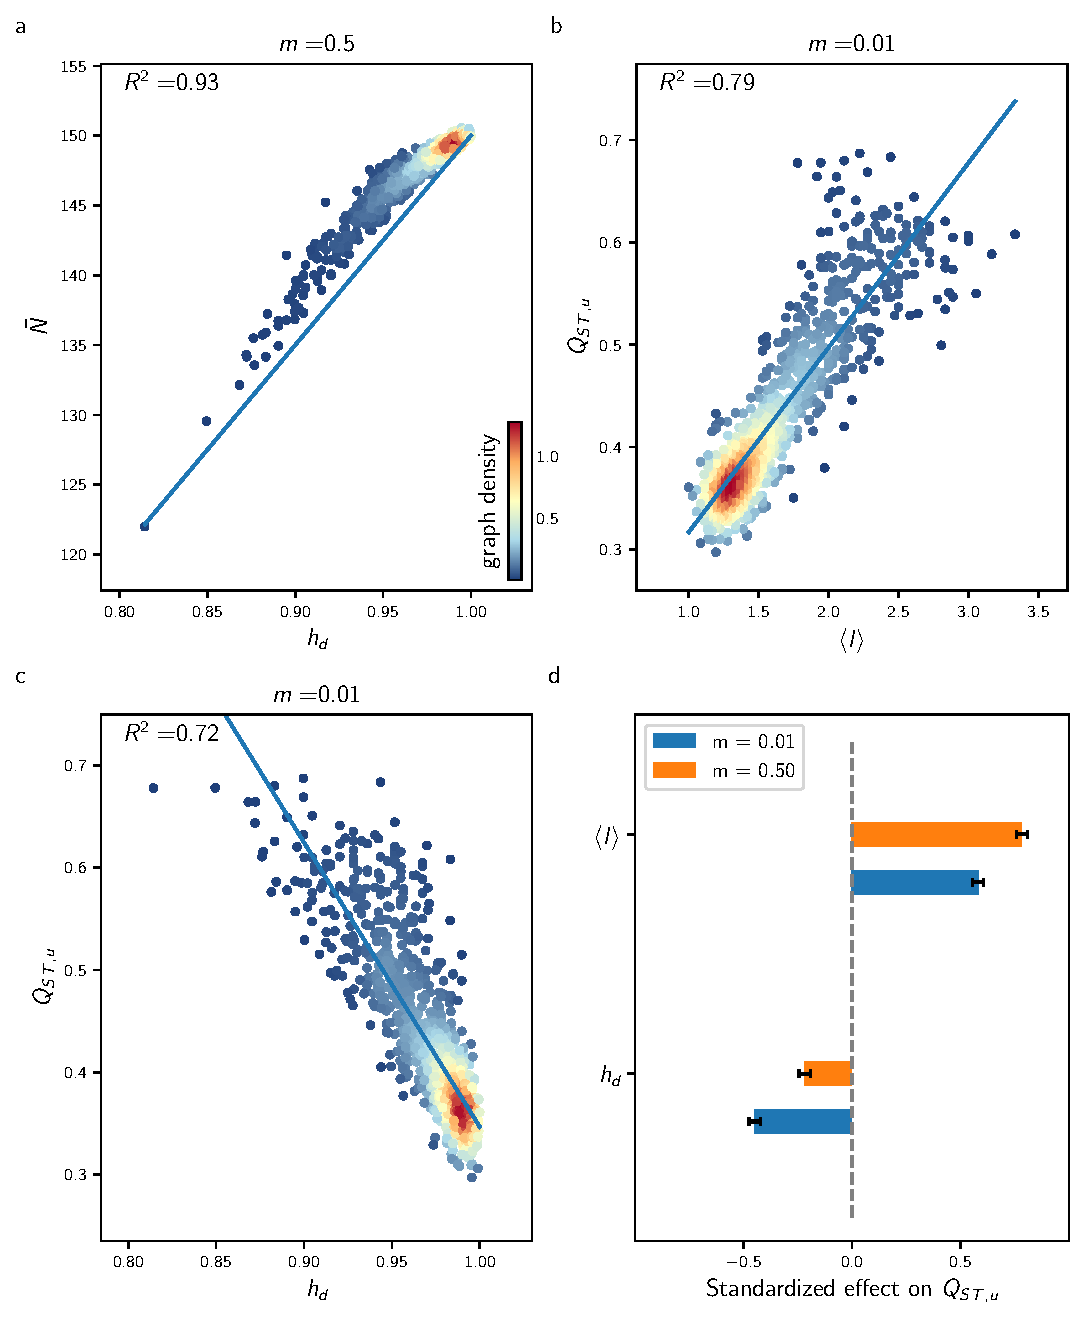
\includegraphics[width=0.8\textwidth]{SI/setting1_neutr_M=9.pdf} 
  }
  \caption{Effect of $\l$ and $h_d$ on average population size $\bar{N}$ and neutral differentiation $Q_{ST,u}$ under the setting with no selection, analogous to \cref{fig:setting1_neutr_M=7} but for 1126 of the 261,080 undirected connected graphs with $M=9$ vertices.}
  \label{figSI:setting1_neutr_M=9}
\end{figure}
\FloatBarrier


\begin{figure}[t]
  \centering
    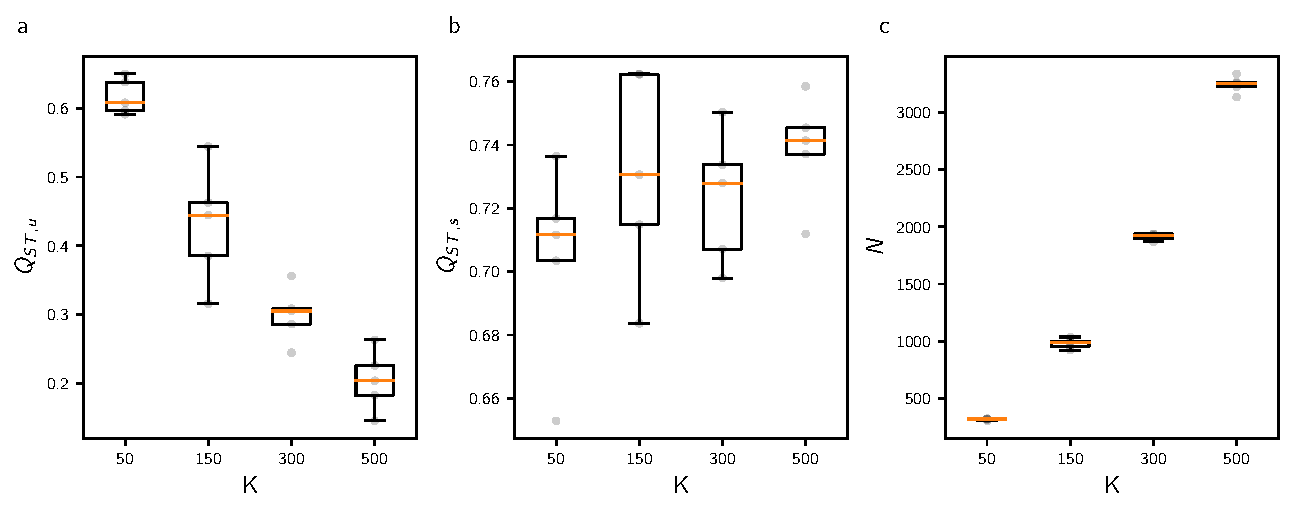
\includegraphics[width=\textwidth]{SI/betau_vs_K.pdf}
    \caption{Effect of the carrying capacity $K$ on $Q_{ST,u}$, $Q_{ST,s}$ and metapopulation size $N$ for the line graph with $M=7$ vertices for $m=0.1$. Decreasing $K$ increases $Q_{ST,u}$ as it favours drift, but it does not influence $Q_{ST,s}$. Each boxplot is based on 5 replicate simulations of the IBM, and fade dots represent single values for each replicate.}\label{figSI:betau_vs_K}
\end{figure}

\FloatBarrier

\begin{figure}[t]
  \centerline{
      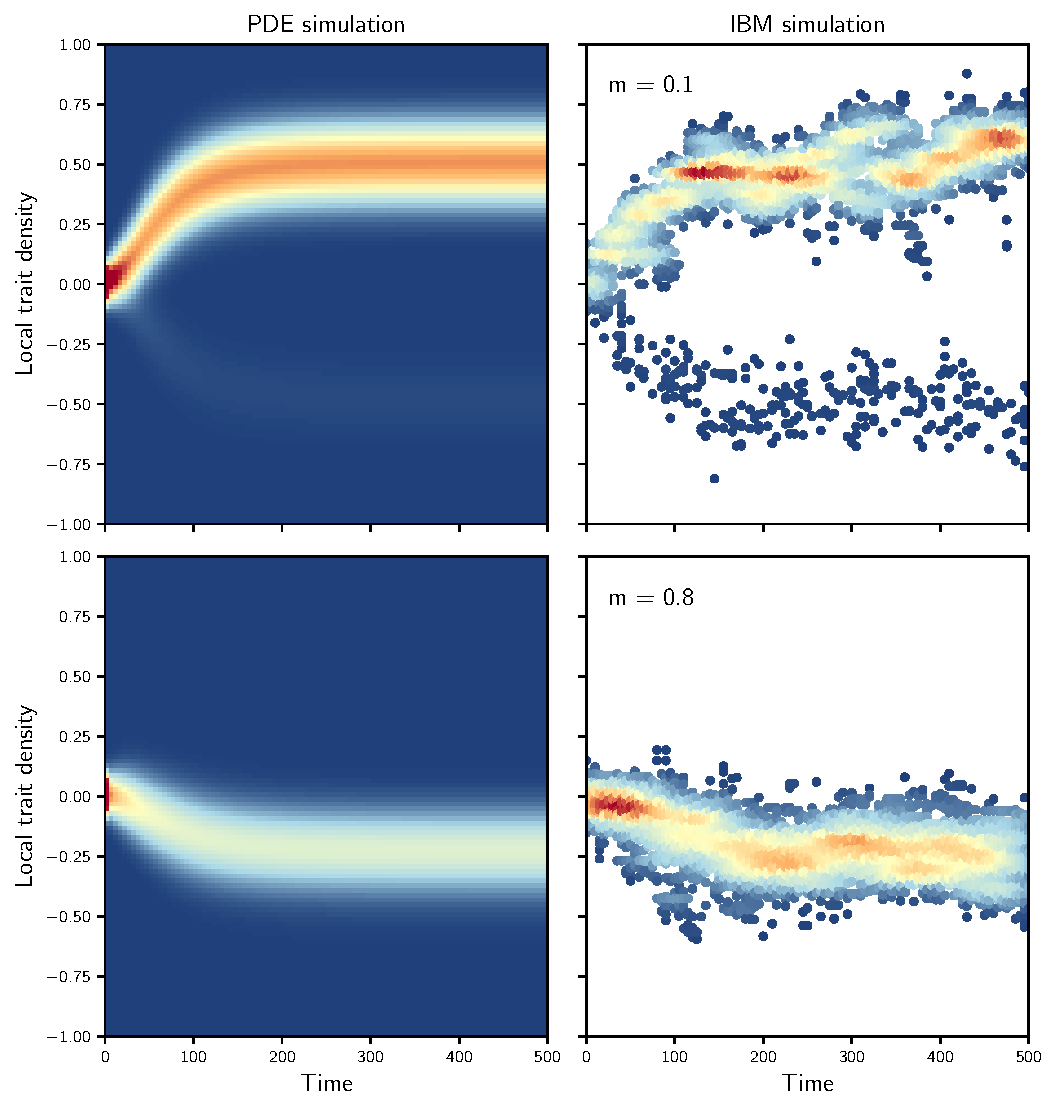
\includegraphics[width=\textwidth,trim= 0 0cm 0cm 0cm]{SI/pde-vs-IBM-trans-setting2_localpop.pdf}}
    \caption{ Comparison of the adaptive trait density on one vertex obtained from \cref{eqSI:PDE_adapt} (left) and from the IBM simulations (right) in the setting with heterogeneous selection, for the star graph with $M=7$ vertices. The densities obtained from \cref{eqSI:PDE_adapt} and from the IBM are qualitatively similar.}
    \label{figSI:pde-vs-IBM-trans-setting2_localpop}
\end{figure}
\FloatBarrier

%%%%%%%%%%%%%%%%%%%%%%%%%%
%%%%%%%%%%PDE vs IBM diversity %%%%%%%%%%%%%
%%%%%%%%%%%%%%%%%%%%%%%%%%

\begin{figure}[t]
  \centering
      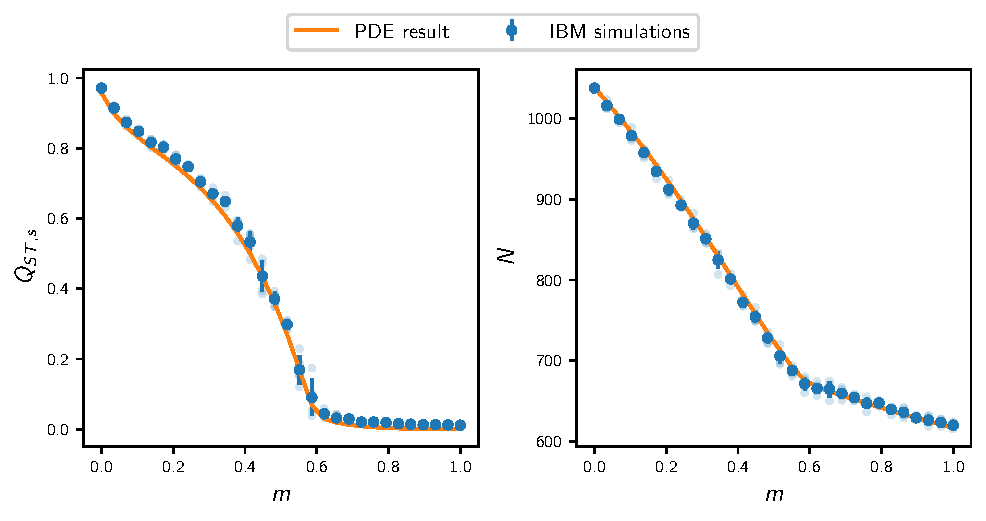
\includegraphics[width=0.8\textwidth,trim= 0 0cm 0cm 0cm]{SI/pde-vs-IBM-mresponse-setting2.pdf}
    \caption{ Comparison of $Q_{ST,s}$ and $N$ obtained from the deterministic approximation \cref{eqSI:PDE_adapt} and from IBM simulations in the setting with heterogeneous selection, on the star graph with $M=7$ vertices. $Q_{ST,s}$ and population size obtained from \cref{eqSI:PDE_adapt} closely match the IBM simulations. Each plain dot represents average results from 5 replicate simulations of the IBM, bars represent one standard deviation, and each fade dot represents a single replicate value.}
    \label{figSI:pde-vs-IBM-mresponse-setting2}
\end{figure}
\FloatBarrier

%%%%%%%%%%%%%%%%%%%%%%%%%%
%%%%%%%%%%r_theta %%%%%%%%%%%%%
%%%%%%%%%%%%%%%%%%%%%%%%%%
\begin{figure}[t]
  \centerline{
      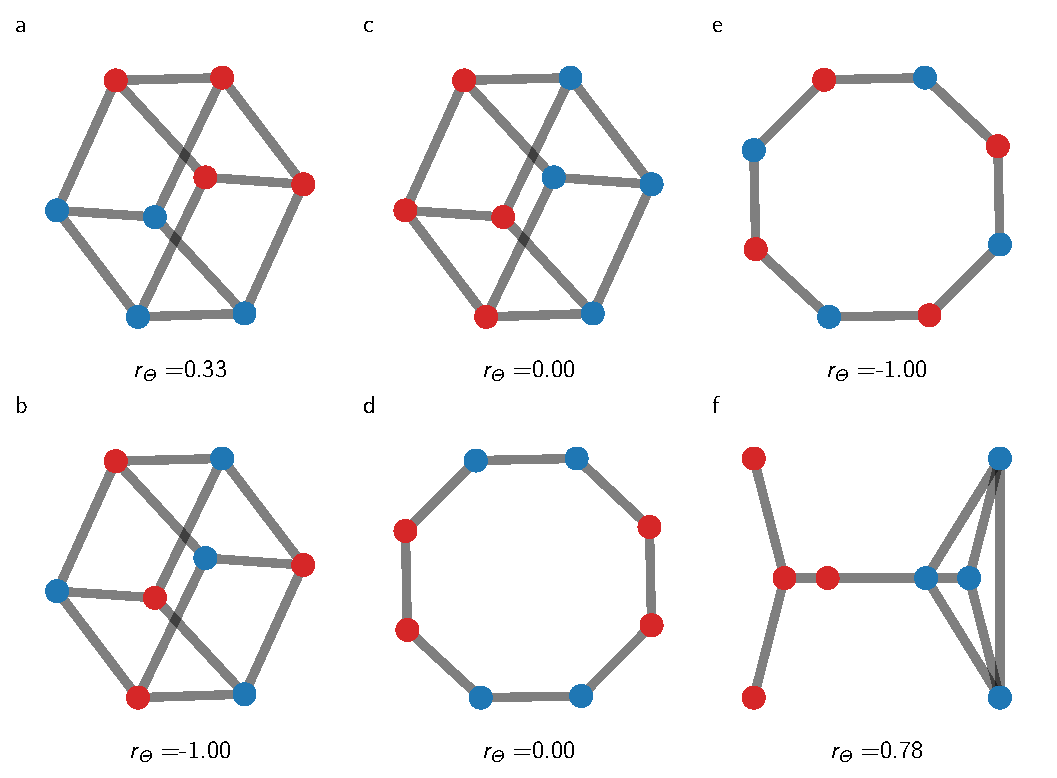
\includegraphics[width=\textwidth]{SI/r_theta_for_different_graphs.pdf} 
  }
  \caption{Graphs with spatial distribution of habitat types corresponding to different habitat assortativity $r_\Theta$. Graphs (a–d) can be described exactly with a mean field approach, as blue and red vertices have an equivalent position on the graph.}
  \label{figSI:graph_rtheta}
\end{figure}
\FloatBarrier

%%%%%%%%%%%%%%%%%%%%%%%%%%
%%%%%%%   PDE m=0.3  %%%%%
%%%%%%%%%%%%%%%%%%%%%%%%%%
\begin{figure}[t]
  \centerline{
      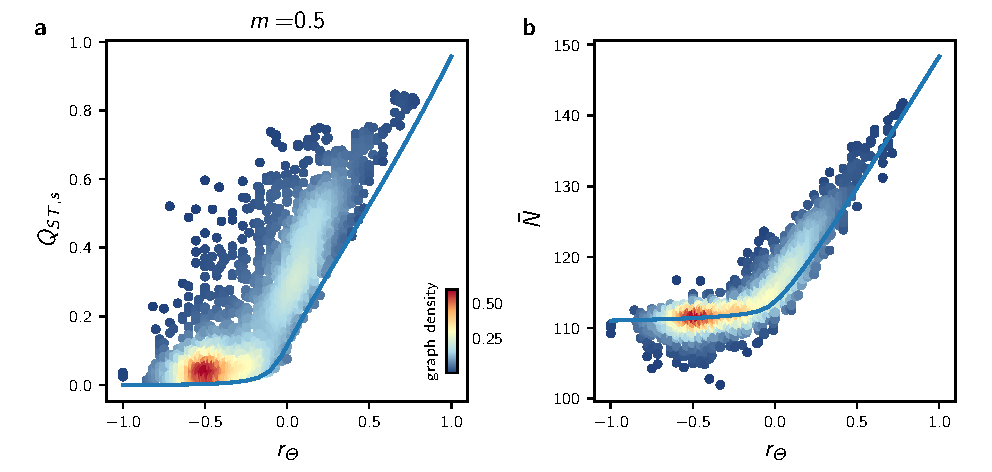
\includegraphics[width=\textwidth]{SI/sett2_adapt_IBM_horizontal_0.5.pdf} 
  }
  \caption{Effects of habitat heterogeneity $r_\Theta$ on $Q_{ST,s}$ and average population size $\bar{N}$ for all undirected connected graphs with $M=7$ vertices and varying $r_\Theta$, obtained for similar simulations to those in \cref{fig:sett2_adapt_IBM_horizontal_0.1} with $m = 0.5$. In (a) and (b), each dot represents average results from 5 replicate simulations of the IBM, the colour scale corresponds to the proportion of the graph with similar $x$ and $y$ axis values (graph density), and the blue lines correspond to results obtained from the mean field, deterministic approximation \cref{eq:PDE_adapt_rtheta}. Deviations from the mean field, deterministic approximation \cref{eq:PDE_adapt_rtheta} can be explained by differences in $\l$ and $h_d$ between the graphs.}
  \label{figSI:sett2_adapt_IBM_horizontal_0.5}
\end{figure}
\FloatBarrier


\begin{figure}[t]
  \centerline{
      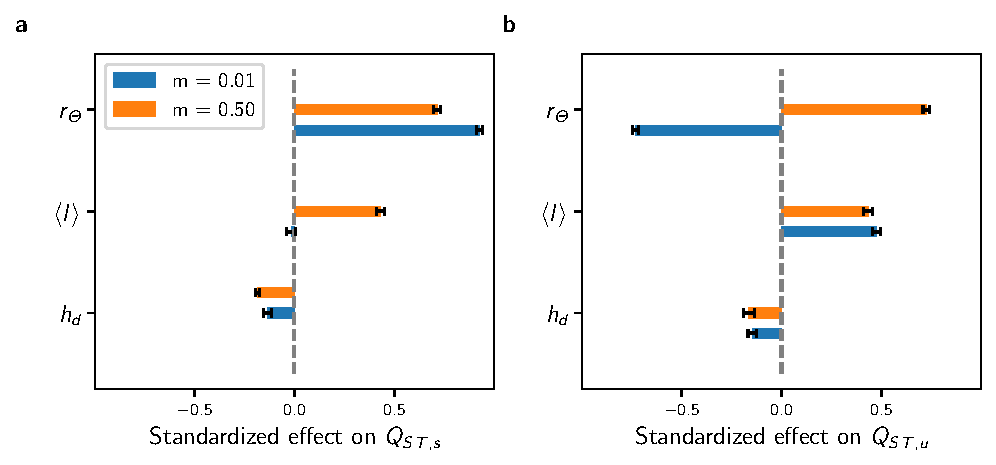
\includegraphics[width=\textwidth]{SI/setting2_2plots_M=9.pdf} 
  }
  \caption{Standardized effects of $h_d$, $\l$ and $r_\Theta$ on $Q_{ST,s}$ and $Q_{ST,u}$ obtained from multivariate regression models independently fitted for low and high migration regimes on average results from 5 replicate simulations of the IBM, analogous \cref{fig:setting2_4plots_M=7}c--d but for 1126 of the 261,080 undirected connected graphs with $M=9$ vertices and varying $r_\Theta$ (see \nameref{sec:methods} for details). Error bars show 95\% confidence intervals.
}
  \label{figSI:setting2_2plots_M=9}
\end{figure}
\FloatBarrier

%%%%%%%%%%%%%%%%%%%%%%%%%%
%%%%%%% real graphs.  %%%%
%%%%%%%%%%%%%%%%%%%%%%%%%%
\begin{figure}[!ht]
  \centerline{
      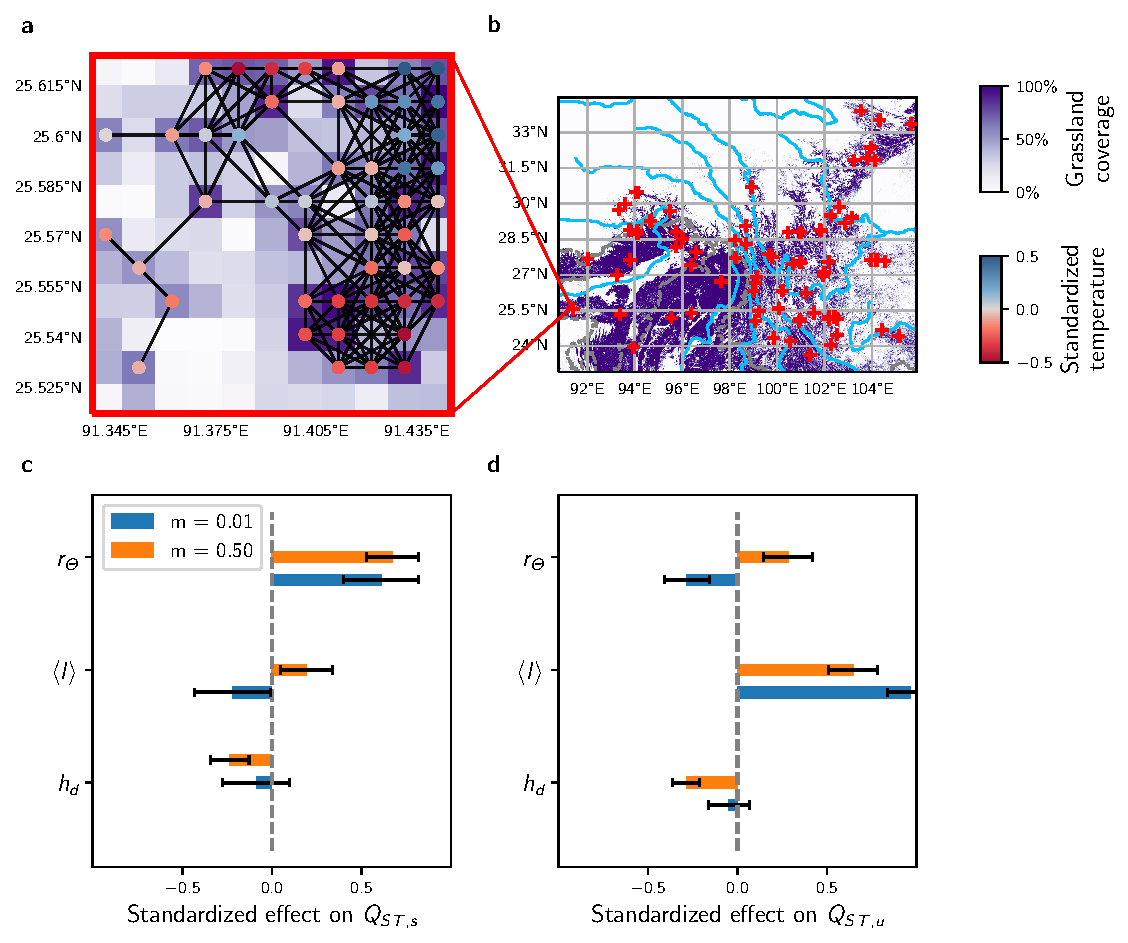
\includegraphics[width=\textwidth]{SI/land2graphs_with_simu.pdf} 
  }
  \caption{\small Simulations on graphs with $M=49$ vertices obtained from real spatial habitat datasets, in the setting with heterogeneous selection. The region from where graphs are obtained is centred on the Hengduan Mountains in Southwest China, one of the most species-rich temperate mountain biota globally \cite{Ding2020a}.
  %
  (a) Graphical representation of a geographical area of size $ 0.11^{\circ} \times 0.11^{\circ}$. To create the graph, we considered biological populations living in grasslands, and used the dataset provided in \cite{Jung2020} containing global grassland coverage at $0.01^\circ$ resolution. We assigned a vertex to a geographical area of size $ 0.01^{\circ} \times 0.01^{\circ}$ if its grassland coverage was above a threshold arbitrarily set to $50\%$. We further assumed that two vertices were connected if their euclidean distance was below a certain dispersal range, which we let vary from 1 to 2.5 km. Local annual average temperature was considered as the value that captures environmental conditions at each vertex. Temperature data was obtained from the CHELSA dataset \cite{Karger2017}.
  %
  (b) Grassland coverage for the considered region. Blue lines correspond to rivers and dashed grey lines correspond to country borders. Red crosses indicate the locations of the 83 graphs sampled for the simulations used in (c--d).
  (c--d) Standardized effects of $h_d$, $\l$ and $r_\Theta$ on $Q_{ST,s}$ and $Q_{ST,u}$ obtained from multivariate regression models independently fitted for low and high migration regimes to average results from 5 replicate simulations of the IBM on the 83 graphs which location is illustrated in (c) (see \cref{tableSI:coefficients_realgraphs} for simulation details). Error bars show 95\% confidence intervals.}
  \label{figSI:graph_real_land}
\end{figure}
\FloatBarrier


\begin{figure}[t]
  \centering
    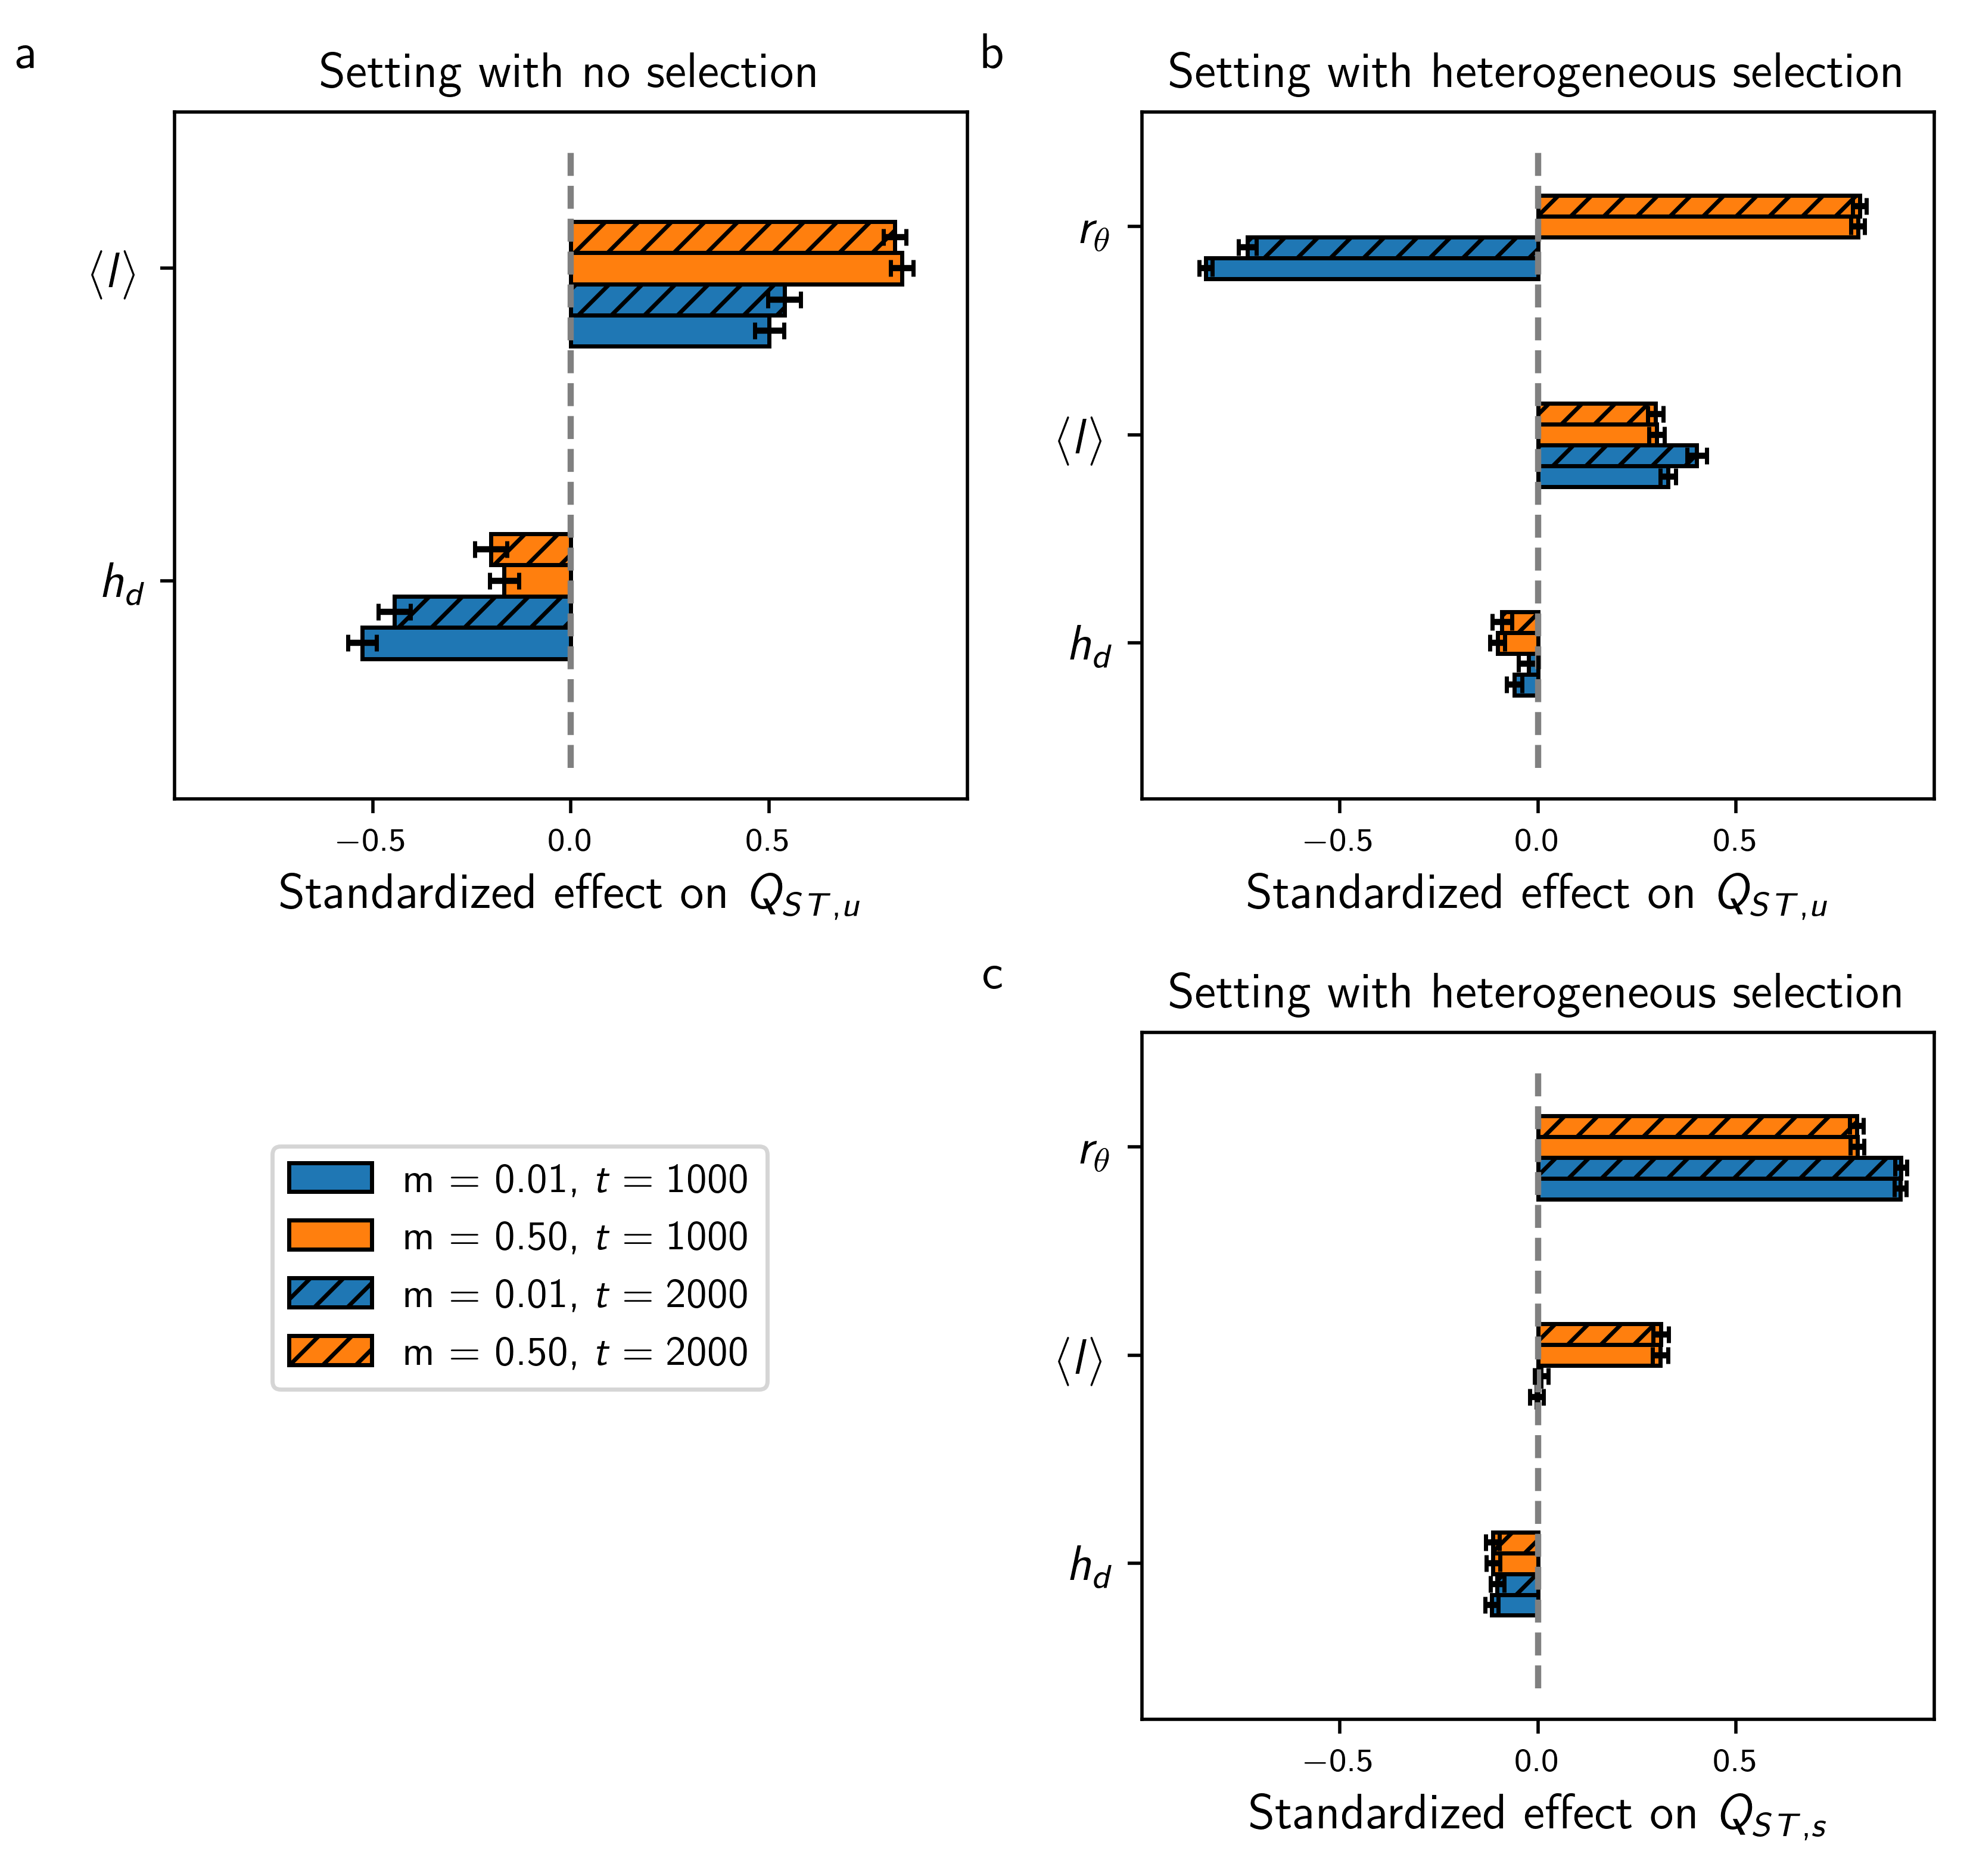
\includegraphics[width=0.9\textwidth]{SI/time_effect_QST_u_QST_s.png}
    \caption{Standardized effects of $h_d$, $\l$ and $r_\Theta$ on $Q_{ST,u}$ in the setting with no selection and in the setting with heterogeneous selection for the time horizons $t=1000$ and $t=2000$, obtained from multivariate regression models independently fitted for low and high migration regimes to average results from 5 replicate simulations of the IBM on all undirected connected graphs with $M=7$ vertices and varying $r_\Theta$ (see \nameref{sec:methods} for details). (a--c) illustrate that the effects of the topology metrics on $Q_{ST,u}$ and  $Q_{ST,s}$ remain constant for $t > 1000$ in both the settings without selection and with heterogeneous selection. Error bars show 95\% confidence intervals. }\label{figSI:time_effect_Q_ST_u}
\end{figure}

\FloatBarrier

\begin{figure}[t]
  \centering
      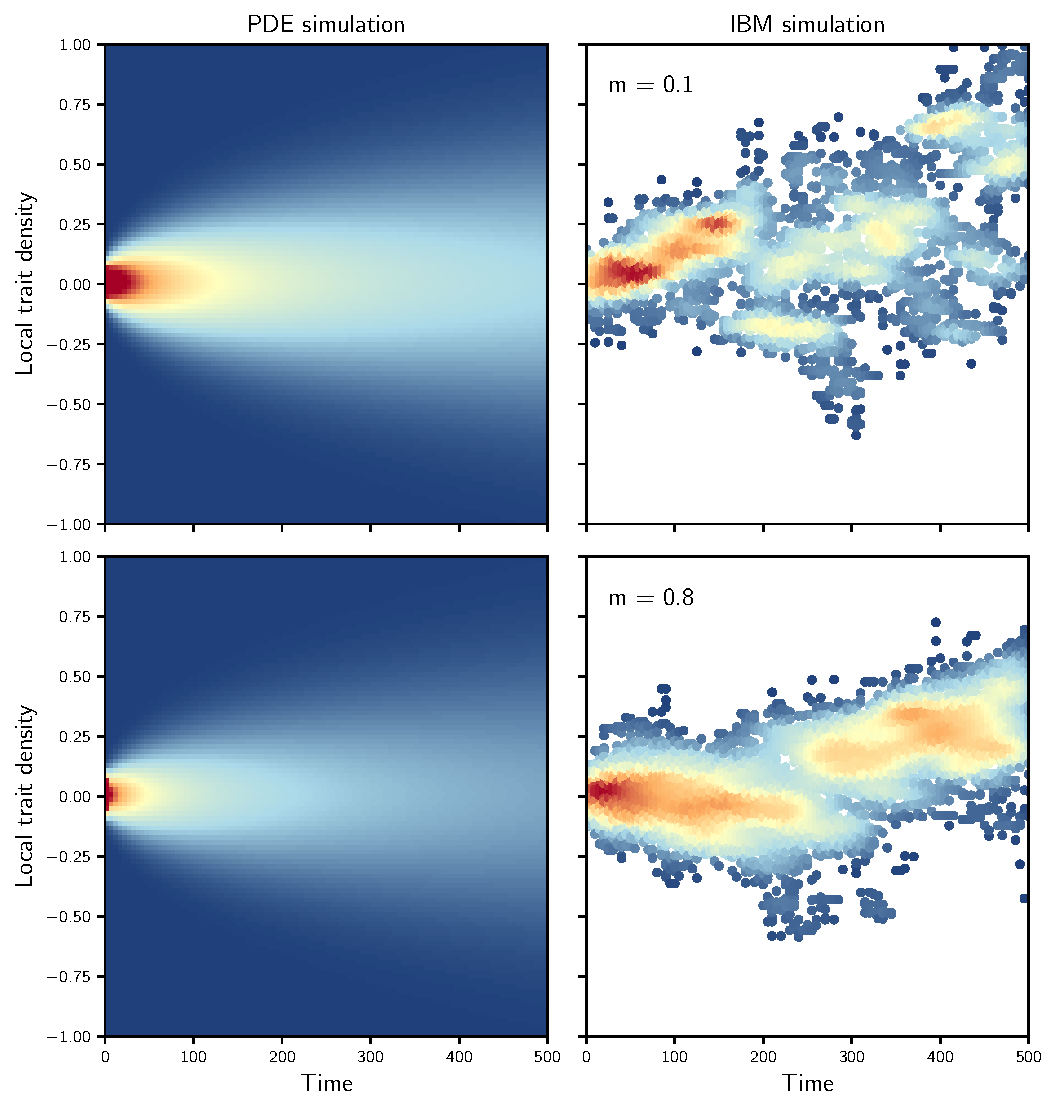
\includegraphics[width=\textwidth]{SI/pde-vs-IBM-trans-setting1_localpop.pdf}
    \caption{ Comparison of the neutral trait density on one vertex obtained from \cref{eqSI:detern_approx_infgen_sett1} (left) and from the IBM simulations (right) in the setting with no selection, for the chain graph. The densities obtained from \cref{eqSI:detern_approx_infgen_sett1} and from the IBM are dissimilar.}
    \label{figSI:pde-vs-IBM-trans-setting1_localpop}
  \end{figure}
\FloatBarrier


\FloatBarrier

\begin{figure}[t]
  \centering
    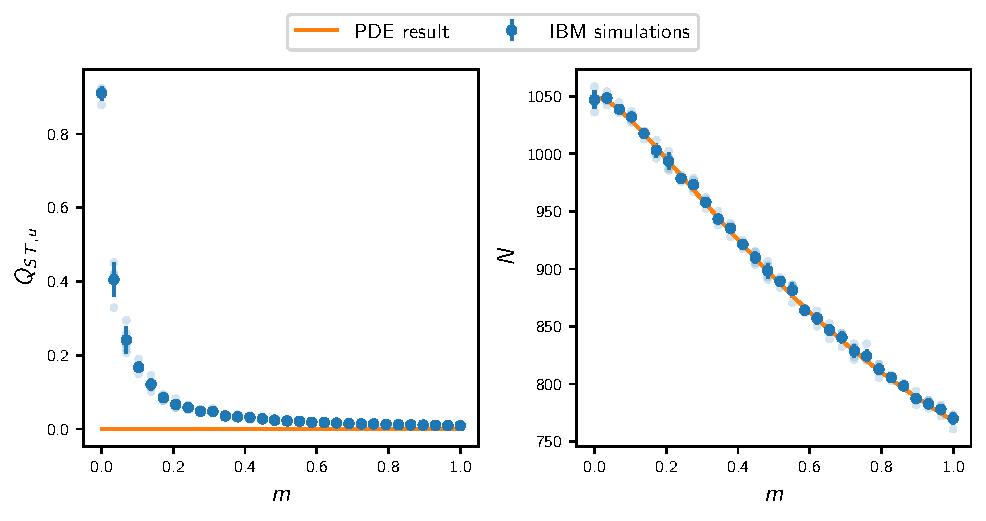
\includegraphics[width=0.8\textwidth]{SI/pde-vs-IBM-mresponse-setting1.pdf} 
    \caption{Comparison of results obtained from the deterministic approximations \cref{eqSI:detern_approx_infgen_sett1,eqSI:sett1_popdyn_simple} and from IBM simulations in the setting with no selection, on the star graph with $M=7$ vertices. While \cref{eqSI:sett1_popdyn_simple} can capture population size, \cref{eqSI:detern_approx_infgen_sett1} is not able to capture $Q_{ST,u}$. Each plain dot represents average results from 5 replicate simulations, bars represent one standard deviation, and each fade dot represents a single replicate value.
    }
    \label{figSI:pde-vs-IBM-mresponse-setting1}
\end{figure}
\clearpage

%%%%%%%%%%%%%%%%%%%%%%%%%%
%%%%%%%%%%tables %%%%%%%%%
%%%%%%%%%%%%%%%%%%%%%%%%%%
\section{Supplementary Tables}
\FloatBarrier

\begin{table}  
  \caption{Linear regression model coefficients for the effect of topology metrics on $Q_{ST,u}$ in the setting with no selection, based on all graphs with $M=7$ vertices. *** $P < 0.001$}
  \vspace{3mm}
  \centering
  % \resizebox{\textwidth}{!}{
    \begin{tabular}{lrrrrrr}
    \toprule
                &  \multicolumn{4}{c}{$Q_{ST,u}$}                                                                          &      \multicolumn{2}{c}{$Q_{ST,u} - b N$}          \\ 
                      \cmidrule(lr){2-5}                                                                                           \cmidrule(lr){6-7}
    $m$         & \multicolumn{1}{c}{0.01} & \multicolumn{1}{c}{0.50} & \multicolumn{1}{c}{0.01} & \multicolumn{1}{c}{0.50} & \multicolumn{1}{c}{0.01} & \multicolumn{1}{c}{0.50} \\ 
    \hline
(Intercept)    &                    0.000 &                   -0.000 &                   -0.000 &                   -0.000 &                   -0.000 &                   -0.000 \\
               &                  (0.023) &                  (0.017) &                  (0.023) &                  (0.025) &                  (0.023) &                  (0.028) \\
$\l$           &                 0.739*** &                 0.872*** &                          &                          &                          &                          \\
               &                  (0.023) &                  (0.017) &                          &                          &                          &                          \\
$h_d$          &                          &                          &                -0.753*** &                -0.674*** &                -0.753*** &                -0.143*** \\
               &                          &                          &                  (0.023) &                  (0.025) &                  (0.023) &                  (0.028) \\
\midrule                                                                                                                                                                           
Number of sim. &                      853 &                      853 &                      853 &                      853 &                      853 &                      853 \\
$R^2$          &                    0.546 &                    0.760 &                    0.567 &                    0.454 &                    0.567 &                    0.030 \\
    \bottomrule
    \end{tabular}
    % }
  \label{tableSI:sett1_1var}
\end{table}
\FloatBarrier

\begin{table}
  \caption{ Multivariate linear regression model coefficients for the effect of topology metrics on $Q_{ST,u}$ in the setting with no selection. *** $P < 0.001$}
  \centering
  % \resizebox{\textwidth}{!}{%
  \begin{tabular}{lrrrr}
    \toprule
    &                                                    \multicolumn{2}{c}{$M=7$} & \multicolumn{2}{c}{$M=9$}                                         \\
    \cmidrule(lr){2-3} \cmidrule(lr){4-5} 
    &                                                    \multicolumn{4}{c}{$Q_{ST,u}$}                                                               \\
     \cmidrule(lr){2-5} 
$m$             & \multicolumn{1}{c}{0.01} & \multicolumn{1}{c}{0.50}  & \multicolumn{1}{c}{0.01} & \multicolumn{1}{c}{0.50} \\
    \hline 
    (Intercept) &                   -0.000 &                   -0.000 &                    0.000 &                   -0.000 \\       
                &                  (0.017) &                  (0.013) &                  (0.009) &                  (0.010) \\       
    $h_d$       &                -0.527*** &                -0.352*** &                -0.449*** &                -0.218*** \\       
                &                  (0.019) &                  (0.014) &                  (0.013) &                  (0.013) \\       
    $\l$        &                 0.500*** &                 0.712*** &                 0.583*** &                 0.784*** \\       
                &                  (0.019) &                  (0.014) &                  (0.013) &                  (0.013) \\       
    \midrule 
Number of sim.  &                      853 &                      853 &                    1,126 &                    1,126 \\       
    $R^2$       &                    0.766 &                    0.858 &                    0.899 &                    0.896 \\       
    \bottomrule
    \end{tabular}
    % }
    \label{tableSI:coefficients_set1}
\end{table}
\FloatBarrier

\begin{table}
  \caption{ Multivariate linear regression model coefficients for the effect of the topology metrics on $Q_{ST,u}$ and $Q_{ST,s}$ in the setting with heterogeneous selection. *** $P < 0.001$}
  \centering
  \resizebox{\textwidth}{!}{
    \begin{tabular}{lrrrrrrrr}
    \toprule
                   & \multicolumn{4}{c}{$M=7$}                                                                                  & \multicolumn{4}{c}{$M=9$}                                                                                   \\                                                                                              
                   \cmidrule(lr){2-5}                                                                                           \cmidrule(lr){6-9}                                                                                             
                   & \multicolumn{2}{c}{$Q_{ST,s}$}    &   \multicolumn{2}{c}{$Q_{ST,u}$}                                        & \multicolumn{2}{c}{$Q_{ST,s}$}    &   \multicolumn{2}{c}{$Q_{ST,u}$}                                         \\
                   \cmidrule(lr){2-3} \cmidrule(lr){4-5}                                                                        \cmidrule(lr){6-7} \cmidrule(lr){8-9}                                                                          
$m$                & \multicolumn{1}{c}{0.01} &  \multicolumn{1}{c}{0.50} & \multicolumn{1}{c}{0.01}& \multicolumn{1}{c}{0.50}   & \multicolumn{1}{c}{0.01} &  \multicolumn{1}{c}{0.50} & \multicolumn{1}{c}{0.01}& \multicolumn{1}{c}{0.50}   \\ 
                   \hline 
    (Intercept)    &                    -0.000 &                   -0.000 &                   -0.000 &                   -0.000   &     0.000 &                    0.000 &                    0.000 &                    0.000\\ 
                   &                   (0.008) &                  (0.009) &                  (0.009) &                  (0.009)   &   (0.008) &                  (0.008) &                  (0.008) &                  (0.008)\\ 
    $h_d$          &                 -0.117*** &                -0.114*** &                -0.060*** &                -0.102***   & -0.135*** &                -0.185*** &                -0.146*** &                -0.164***\\ 
                   &                   (0.009) &                  (0.010) &                  (0.010) &                  (0.010)   &   (0.010) &                  (0.011) &                  (0.011) &                  (0.011)\\ 
    $\l$           &                    -0.004 &                 0.308*** &                 0.328*** &                 0.300***   &    -0.017 &                 0.431*** &                 0.475*** &                 0.434***\\ 
                   &                   (0.009) &                  (0.010) &                  (0.010) &                  (0.010)   &   (0.010) &                  (0.011) &                  (0.011) &                  (0.011)\\ 
    $r_\Theta$     &                  0.914*** &                 0.805*** &                -0.838*** &                 0.807***   &  0.926*** &                 0.715*** &                -0.730*** &                 0.725***\\ 
                   &                   (0.008) &                  (0.009) &                  (0.009) &                  (0.009)   &   (0.008) &                  (0.008) &                  (0.008) &                  (0.008)\\ 
    \midrule
    Number of sim. &                     2,548 &                    2,548 &                    2,548 &                    2,548   &     2,250 &                    2,250 &                    2,250 &                    2,250\\ 
    $R^2$          &                     0.845 &                    0.808 &                    0.808 &                    0.799   &     0.870 &                    0.853 &                    0.862 &                    0.851\\ 
    \bottomrule
    \end{tabular}
    }
    \label{tableSI:coefficients_set2}
\end{table}
\FloatBarrier

\begin{table}
  \caption{Multivariate linear regression model coefficients for the effect of topology metrics on $Q_{ST,u}$ and $Q_{ST,s}$ on real graphs with $M=49$ vertices in the setting with heterogeneous selection. * $P < 0.05$,  ** $P < 0.01$, *** $P < 0.001$}
  \centering
  % \resizebox{\textwidth}{!}{%
  % \resizebox{\textwidth}{!}{
    \begin{tabular}{lrrrr}
    \toprule
    &       \multicolumn{2}{c}{$Q_{ST,s}$}                           &               \multicolumn{2}{c}{$Q_{ST,u}$}        \\ 
    \cmidrule(lr){2-3} \cmidrule(lr){4-5} 
$m$            & \multicolumn{1}{c}{0.1} & \multicolumn{1}{c}{0.50} & \multicolumn{1}{c}{0.1} & \multicolumn{1}{c}{0.50} \\ 
    \hline
(Intercept) &                  -0.000 &                   -0.000 &                    0.000 &                   -0.000 \\ 
            &                 (0.093) &                  (0.064) &                  (0.056) &                  (0.059) \\ 
$h_d$       &                  -0.088 &                -0.235*** &                   -0.048 &                -0.286*** \\ 
            &                 (0.094) &                  (0.065) &                  (0.057) &                  (0.060) \\ 
$\l$        &                 -0.220* &                  0.195** &                 0.965*** &                 0.645*** \\ 
            &                 (0.106) &                  (0.073) &                  (0.064) &                  (0.068) \\ 
$r_\Theta$  &                0.610*** &                 0.675*** &                -0.282*** &                 0.282*** \\ 
            &                 (0.106) &                  (0.073) &                  (0.063) &                  (0.068) \\ 
\midrule
Number of sim.&                    83 &                       83 &                       83 &                       83 \\ 
$R^2$       &                   0.313 &                    0.675 &                    0.752 &                    0.717 \\ 
    \bottomrule
  \end{tabular}
  % }
\label{tableSI:coefficients_realgraphs}
\end{table}
\FloatBarrier


\begin{table}
  \caption{ Multivariate linear regression model coefficients for the effect of topology metrics on $Q_{ST,u}$ and $Q_{ST,s}$ in the setting of trait-dependent competition and heterogeneous selection (\cref{secSI:trait-dep-comp}), based on all graphs with $M=7$ vertices.  *** $P < 0.001$}
  \centering
  % \resizebox{\textwidth}{!}{%
  \resizebox{\textwidth}{!}{\begin{tabular}{lrrrrrrrr}
    \toprule
                &                                 \multicolumn{4}{c}{$\sigma_a = 0.5 < \nicefrac{1}{\sqrt{2p}}$} & \multicolumn{4}{c}{$\sigma_a = 1 > \nicefrac{1}{\sqrt{2p}}$} \\
                \cmidrule(lr){2-5} \cmidrule(lr){6-9} 
                &            \multicolumn{2}{c}{$Q_{ST,s}$}           &            \multicolumn{2}{c}{$Q_{ST,u}$}           &            \multicolumn{2}{c}{$Q_{ST,s}$}           &            \multicolumn{2}{c}{$Q_{ST,u}$}          \\ 
                \cmidrule(lr){2-3} \cmidrule(lr){4-5} \cmidrule(lr){6-7} \cmidrule(lr){8-9} 
    $m$          & \multicolumn{1}{c}{0.05} & \multicolumn{1}{c}{0.50} & \multicolumn{1}{c}{0.05} & \multicolumn{1}{c}{0.50} & \multicolumn{1}{c}{0.05} & \multicolumn{1}{c}{0.50} & \multicolumn{1}{c}{0.05} & \multicolumn{1}{c}{0.50}\\ 
    \hline
    (Intercept) &                    0.000 &                   -0.000 &                   -0.000 &                   -0.000 &                    0.000 &                   -0.000 &                    0.000 &                   -0.000\\ 
                &                  (0.005) &                  (0.010) &                  (0.011) &                  (0.010) &                  (0.004) &                  (0.008) &                  (0.012) &                  (0.007)\\ 
    $h_d$       &                -0.228*** &                -0.118*** &                -0.171*** &                -0.169*** &                -0.166*** &                -0.128*** &                -0.178*** &                -0.139***\\ 
                &                  (0.006) &                  (0.011) &                  (0.012) &                  (0.012) &                  (0.004) &                  (0.009) &                  (0.013) &                  (0.008)\\ 
    $\l$        &                 0.084*** &                 0.373*** &                 0.461*** &                 0.573*** &                    0.002 &                 0.296*** &                 0.483*** &                 0.286***\\ 
                &                  (0.006) &                  (0.011) &                  (0.012) &                  (0.012) &                  (0.004) &                  (0.009) &                  (0.013) &                  (0.008)\\ 
    $r_\Theta$  &                 0.922*** &                 0.741*** &                -0.657*** &                 0.508*** &                 0.967*** &                 0.816*** &                -0.585*** &                 0.837***\\ 
                &                  (0.005) &                  (0.010) &                  (0.011) &                  (0.010) &                  (0.004) &                  (0.008) &                  (0.012) &                  (0.007)\\ 
    \hline
Number of sim.  &                    2,548 &                    2,548 &                    2,548 &                    2,548 &                    2,548 &                    2,548 &                    2,548 &                    2,548\\ 
    $R^2$       &                    0.934 &                    0.768 &                    0.716 &                    0.732 &                    0.962 &                    0.828 &                    0.659 &                    0.861\\ 
    \bottomrule
    \end{tabular}}
\label{tableSI:coefficients_trait-dep-comp}
\end{table}

